\documentclass[conference]{IEEEtran}
\IEEEoverridecommandlockouts

\usepackage{cite}
\usepackage{amsmath,amssymb}
\usepackage{graphicx}
\usepackage{booktabs}
\usepackage{multirow}
\usepackage{array}
\usepackage{xcolor}
\usepackage{tikz}
\usetikzlibrary{arrows.meta,positioning}
\usepackage{algorithm}
\usepackage{algpseudocode}
\usepackage{url}
\usepackage[colorlinks=true,linkcolor=black,citecolor=black,urlcolor=blue!70!black,
            pdftitle={MeetingMind: An End-to-End Generative AI System for Evidence-Grounded Meeting Intelligence},
            pdfauthor={Deon Menezes, Aishwarya Gawali},
            pdfsubject={Generative AI Laboratory - Mini Project},
            pdfkeywords={speech recognition, speaker diarization, large language models, retrieval-augmented generation}]{hyperref}

\newcommand{\repo}{\href{https://github.com/DeonMenezes-11/MeetingMind}{\nolinkurl{github.com/DeonMenezes-11/MeetingMind}}}

\begin{document}

\title{MeetingMind: An End-to-End Generative AI System for Evidence-Grounded Meeting Intelligence}

\author{\IEEEauthorblockN{Deon Menezes}
\IEEEauthorblockA{\textit{Dept. of Artificial Intelligence and Data Science}\\
\textit{K. J. Somaiya School of Engineering}\\
\textit{Somaiya Vidyavihar University}, Mumbai, India\\
Roll No. 16014223030}
\and
\IEEEauthorblockN{Aishwarya Gawali}
\IEEEauthorblockA{\textit{Dept. of Artificial Intelligence and Data Science}\\
\textit{K. J. Somaiya School of Engineering}\\
\textit{Somaiya Vidyavihar University}, Mumbai, India\\
Roll No. 16014223007}}

\maketitle

\begin{abstract}
Decisions and commitments made in meetings are easily lost, and minutes written by a language model are only useful if every
item can be traced back to what was actually said. We present \emph{MeetingMind}, an end-to-end generative AI application that
turns a meeting recording into a speaker-attributed transcript, structured minutes whose decisions and action items are verified
against the transcript, per-owner follow-up emails, and a retrieval-augmented question-answering assistant that cites playable
timestamps and refuses questions the meeting never addressed. The pipeline combines a diarizing speech model, a
\emph{self-enrolment} second pass that uses each participant's own introduction as a voice reference, schema-constrained
generation that cites segment identifiers instead of times, a deterministic evidence checker, and a hybrid embedding retriever
with two refusal gates. A FastAPI back end exposes the pipeline as background jobs with live progress, and a React front end
keeps a human in the loop. On a scripted four-speaker meeting with exact gold labels, MeetingMind reaches 4.0\% word error rate,
100\% time-weighted speaker attribution (up from 80.5\% without self-enrolment), and perfect action-item precision and recall;
with 10\,dB background noise it keeps 3.5\% WER, 92.6\% attribution and 0.875 recall, while every reported item passes the
evidence check. Processing a 5\,min 20\,s meeting costs about US\$0.065. The source code is available at \repo.
\end{abstract}

\begin{IEEEkeywords}
speech recognition, speaker diarization, large language models, structured outputs, retrieval-augmented generation,
hallucination, prompt injection, human-in-the-loop
\end{IEEEkeywords}

\section{Introduction}
Meetings are where teams decide what to build and who will do it, yet the outcome usually survives only as memory or as notes
taken by one participant. Speech recognition and large language models (LLMs) make automatic minutes possible, but two problems
make naive ``transcribe, then summarise'' pipelines hard to trust. First, an LLM can attribute a task to the wrong person or
invent a deadline~\cite{ji2023hallucination}, and a reader cannot tell which items are real. Second, the transcript is text
spoken by people, so it can contain instructions aimed at the model (\emph{indirect prompt injection}~\cite{greshake2023}).

This paper describes MeetingMind, a complete application built as the mini project of a Generative AI laboratory course. Our
contributions are:
\begin{itemize}
  \item an end-to-end pipeline from raw audio to verified minutes, emails and cited question answering, with per-stage caching,
        latency and cost accounting;
  \item \emph{self-enrolment diarization}: when self-introductions contradict the diarizer's speaker labels, each person's
        introduction is reused as a reference clip for a second pass, raising speaker attribution from 80.5\% to 100\%;
  \item a grounding contract in which the LLM cites segment IDs and verbatim quotes that deterministic code verifies, so every
        item is either verified or visibly flagged;
  \item retrieval-augmented question answering with two refusal gates (a similarity threshold and an explicit
        \texttt{NOT\_FOUND} reply);
  \item a web application (FastAPI + React) with live progress, a shared audio player and human review of action items; and
  \item an algorithmic evaluation against a synthesised meeting with an exact gold timeline, including a noisy variant and a
        spoken prompt-injection attempt.
\end{itemize}
The implementation, tests, sample data and this report are publicly available on GitHub:\\ \repo.

\section{Related Work}
\textbf{Speech recognition.} Transformer encoder--decoder models~\cite{vaswani2017} trained on large weakly supervised corpora,
such as Whisper~\cite{radford2023whisper}, are robust to accents and noise without domain fine-tuning; the GPT-4o transcription
models used here follow the same design with a larger language-model decoder.

\textbf{Speaker diarization} answers ``who spoke when''. Classical systems cluster speaker embeddings such as
x-vectors~\cite{snyder2018xvectors}; neural toolkits such as pyannote~\cite{bredin2020pyannote} and end-to-end neural
diarization~\cite{fujita2019eend} handle overlap better. Park \emph{et al.}~\cite{park2022review} survey the field; confusion
between similar voices remains a dominant error, which motivates our enrolment pass.

\textbf{Meeting summarisation.} The AMI corpus~\cite{carletta2005ami} and QMSum~\cite{zhong2021qmsum} established meeting
summarisation and query-based summarisation as tasks. LLMs~\cite{brown2020gpt3} now perform them zero-shot, but
hallucination~\cite{ji2023hallucination} makes verification essential.

\textbf{Retrieval augmentation and safety.} Retrieval-augmented generation (RAG)~\cite{lewis2020rag} conditions answers on
retrieved passages, typically found with dense embeddings~\cite{karpukhin2020dpr}. Greshake \emph{et al.}~\cite{greshake2023}
showed that text processed by an LLM application can hijack it; meeting transcripts are exactly such untrusted input.

\section{System Architecture}
Fig.~\ref{fig:arch} shows the pipeline. An orchestrator runs eight stages, caches every intermediate artefact under
\texttt{runs/<id>/} and records per-stage latency, token usage and estimated cost, so repeated runs never repeat paid calls.

\begin{figure*}[t]
  \centering
  \resizebox{\textwidth}{!}{% MeetingMind pipeline (TikZ) - included by meetingmind_ieee.tex
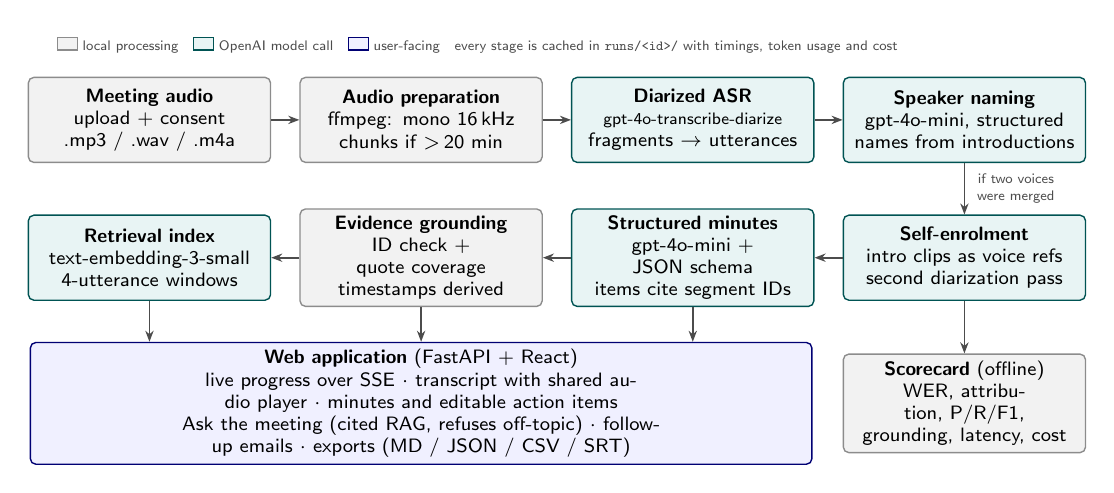
\begin{tikzpicture}[
  font=\sffamily\scriptsize, >={Stealth[length=4pt]},
  box/.style={draw, rounded corners=2pt, align=center, minimum height=1.08cm, text width=2.9cm, inner sep=2.5pt, line width=0.5pt},
  local/.style={box, fill=black!5, draw=black!45},
  ai/.style={box, fill=teal!9, draw=teal!65!black},
  ui/.style={box, fill=blue!6, draw=blue!45!black},
  arr/.style={->, line width=0.6pt, draw=black!70},
  lbl/.style={font=\sffamily\tiny, text=black!70, align=center},
]
% row 1
\node[local] (audio) at (0,0)    {\textbf{Meeting audio}\\upload + consent\\.mp3 / .wav / .m4a};
\node[local] (prep)  at (3.45,0)  {\textbf{Audio preparation}\\ffmpeg: mono 16\,kHz\\chunks if $>$\,20 min};
\node[ai]    (asr)   at (6.9,0)  {\textbf{Diarized ASR}\\{\fontsize{6.4}{7}\selectfont gpt-4o-transcribe-diarize}\\fragments $\rightarrow$ utterances};
\node[ai]    (names) at (10.35,0)  {\textbf{Speaker naming}\\gpt-4o-mini, structured\\names from introductions};
% row 2
\node[ai]    (enrol) at (10.35,-1.75) {\textbf{Self-enrolment}\\intro clips as voice refs\\second diarization pass};
\node[ai]    (min)   at (6.9,-1.75) {\textbf{Structured minutes}\\gpt-4o-mini + JSON schema\\items cite segment IDs};
\node[local] (gr)    at (3.45,-1.75) {\textbf{Evidence grounding}\\ID check + quote coverage\\timestamps derived};
\node[ai]    (idx)   at (0,-1.75)   {\textbf{Retrieval index}\\text-embedding-3-small\\4-utterance windows};
% row 3
\node[ui, text width=9.75cm, minimum height=1.0cm] (web) at (3.45,-3.6)
  {\textbf{Web application} (FastAPI + React)\\live progress over SSE $\cdot$ transcript with shared audio player $\cdot$ minutes and editable action items\\Ask the meeting (cited RAG, refuses off-topic) $\cdot$ follow-up emails $\cdot$ exports (MD / JSON / CSV / SRT)};
\node[local] (score) at (10.35,-3.6) {\textbf{Scorecard} (offline)\\WER, attribution, P/R/F1,\\grounding, latency, cost};
% arrows
\draw[arr] (audio) -- (prep);
\draw[arr] (prep) -- (asr);
\draw[arr] (asr) -- (names);
\draw[arr] (names) -- node[right, lbl, xshift=1pt]{if two voices\\were merged} (enrol);
\draw[arr] (enrol) -- (min);
\draw[arr] (min) -- (gr);
\draw[arr] (gr) -- (idx);
\draw[arr] (idx.south) -- (idx.south |- web.north);
\draw[arr] (gr.south) -- (gr.south |- web.north);
\draw[arr] (min.south) -- (min.south |- web.north);
\draw[arr] (enrol.south) -- (score.north);
% legend
\node[lbl, anchor=west] at (-1.3,0.95) {\tikz\draw[fill=black!5, draw=black!45] (0,0) rectangle (0.25,0.16);~local processing\quad
  \tikz\draw[fill=teal!9, draw=teal!65!black] (0,0) rectangle (0.25,0.16);~OpenAI model call\quad
  \tikz\draw[fill=blue!6, draw=blue!45!black] (0,0) rectangle (0.25,0.16);~user-facing\quad
  every stage is cached in \texttt{runs/<id>/} with timings, token usage and cost};
\end{tikzpicture}
}
  \caption{MeetingMind pipeline. Model calls (teal) are wrapped by local, deterministic stages (grey) that prepare audio and
  verify outputs; the web application (blue) presents the results and keeps a human in the loop.}
  \label{fig:arch}
\end{figure*}

\subsection{Audio preparation and diarized transcription}
\texttt{ffprobe} measures the recording and \texttt{ffmpeg} normalises it to mono 16\,kHz, 64\,kbit/s MP3, with a 25\,MB guard;
recordings longer than 20 minutes are split into 10-minute chunks whose offsets are measured rather than assumed. The audio is
transcribed by \texttt{gpt-4o-transcribe-diarize} (\texttt{diarized\_json}, server-side chunking), which returns phrase-level
fragments with anonymous speaker labels (A, B, \dots). Consecutive fragments of the same speaker are merged into utterances
$S_1,\dots,S_n$ (117 fragments became 47 utterances in our sample). If diarization is unavailable the system falls back to
\texttt{whisper-1} without speaker labels and says so in the interface.

\subsection{Speaker naming and self-enrolment}
\texttt{gpt-4o-mini} receives the opening utterances and returns, through a strict schema, a mapping from labels to names and
roles together with the list of self-introductions (``Hi, I'm Rohan, the back-end developer''). A name is accepted only if it
occurs in the cited utterance; an optional participant list corrects recogniser spellings (``Mira''~$\rightarrow$~``Meera'') by
requiring the same initial and a string-similarity ratio of at least 0.65.

In the first pass the diarizer merged two of the four voices: a single label covered both Priya's and Meera's introductions. The
\emph{self-enrolment} step detects exactly this contradiction, cuts a 2--6\,s clip of each person's introduction and re-runs
diarization with those clips as \texttt{known\_speaker\_references}. The second pass labels utterances directly with names.
Because it needs introductions and supports at most four reference speakers, it runs only when the contradiction is detected.

\subsection{Structured minutes with segment citations}
The transcript is rendered as lines such as \texttt{[S12 03:41 Priya] \dots} inside \texttt{<transcript>} tags. The system
prompt states that the transcript is untrusted data whose embedded instructions must be ignored, while genuine tasks in the same
utterance must still be extracted. Using structured outputs, the model returns a \texttt{Minutes} object: title, executive
summary, topics (start and end segment IDs), decisions, action items (owner, task, due date, priority), open questions and
risks. Every item carries \texttt{evidence\_segment\_ids} and a verbatim \texttt{evidence\_quote}. The schema deliberately has
no timestamp fields: the model cites IDs, and times are derived from the transcript by code.

\subsection{Evidence grounding}
Algorithm~\ref{alg:ground} verifies each decision, action item, question and risk. Items that fail are kept but flagged for
review, excluded from follow-up emails by default, and shown with a warning badge in the interface.

\begin{algorithm}[t]
\caption{Evidence grounding of one minutes item}
\label{alg:ground}
\begin{algorithmic}[1]
\Require item with cited IDs $C$ and quote $q$; utterances $\{S_i\}$
\State $V \gets \{c \in C \mid c \text{ is a valid utterance ID}\}$
\If{$V = \emptyset$} \State \Return \textsc{ungrounded}(``no valid evidence'') \EndIf
\State $\kappa \gets \textsc{Coverage}(q, \text{text}(V))$ \Comment{longest matching blocks / $|q|$}
\If{$\kappa < 0.6$}
  \State $V' \gets V \cup \text{neighbours}(V)$ \Comment{quote may run into the next utterance}
  \If{$\textsc{Coverage}(q, \text{text}(V')) \ge 0.6$} \State $V \gets V'$; mark \emph{repaired} \Else \State \Return \textsc{ungrounded} \EndIf
\EndIf
\State $t \gets \min_{v \in V} \text{start}(S_v)$ \Comment{timestamp derived, never generated}
\State \Return \textsc{grounded}$(V, t, \kappa)$
\end{algorithmic}
\end{algorithm}

\subsection{Ask the meeting}
The transcript is cut into windows of four utterances with an overlap of one (16 windows for the sample) and embedded with
\texttt{text-embedding-3-small}. A question is embedded and windows are ranked by cosine similarity plus a small keyword bonus
($0.15\times$ the share of the question's content words found in the window), which helps with names and dates. Two gates
prevent answers that are not in the meeting: if the best cosine is below 0.25 the LLM is not called at all, and otherwise the
model must reply \texttt{NOT\_FOUND} when the retrieved excerpts do not contain the answer. Answers must cite the
\texttt{[mm:ss]} timestamps of the excerpts, and citations are validated against the retrieved windows.

\subsection{Follow-up emails}
Emails are generated from the human-reviewed action items, either by a deterministic template or by one structured LLM call in a
formal or friendly tone. Only items that are verified or explicitly approved by the reviewer are included, recipients that do
not exist in the reviewed table are dropped, and emails are drafts that a person sends.

\section{Web Application}
\label{sec:web}
The pipeline is served by a FastAPI back end and a React~19 / TypeScript / Tailwind front end built with Vite.

\textbf{Back end.} Uploads are validated (consent flag, file type, 200\,MB limit) and become background jobs; one pipeline runs at
a time and further jobs queue. The orchestrator's progress callback appends events that the browser receives through
server-sent events, so a four-minute job shows each stage, its sub-steps and timings live (Fig.~\ref{fig:process}). Audio is served
with HTTP range support so the player can seek, speaker renames and edited action items are stored per meeting, and every export
(Markdown, JSON, CSV, SRT) is a download. The API key stays on the server and the server binds to \texttt{localhost} by default.

\textbf{Front end.} A home page lists processed meetings; an upload page guides the user through file selection, an optional
participant list and a consent step, explaining what is still missing. The meeting workspace (Fig.~\ref{fig:overview}) has six
sections that share one audio player whose scrubber is coloured by speaker: an overview with a clickable agenda, outcome
counts, a topic timeline and decisions with their evidence; a transcript in which clicking a line plays it and the current
line is followed during playback; editable action items; the question-answering chat; follow-up emails; and analytics
(Fig.~\ref{fig:screens}). The interface supports light and dark themes, phone-width layouts and keyboard shortcuts.

\begin{figure*}[t]
  \centering
  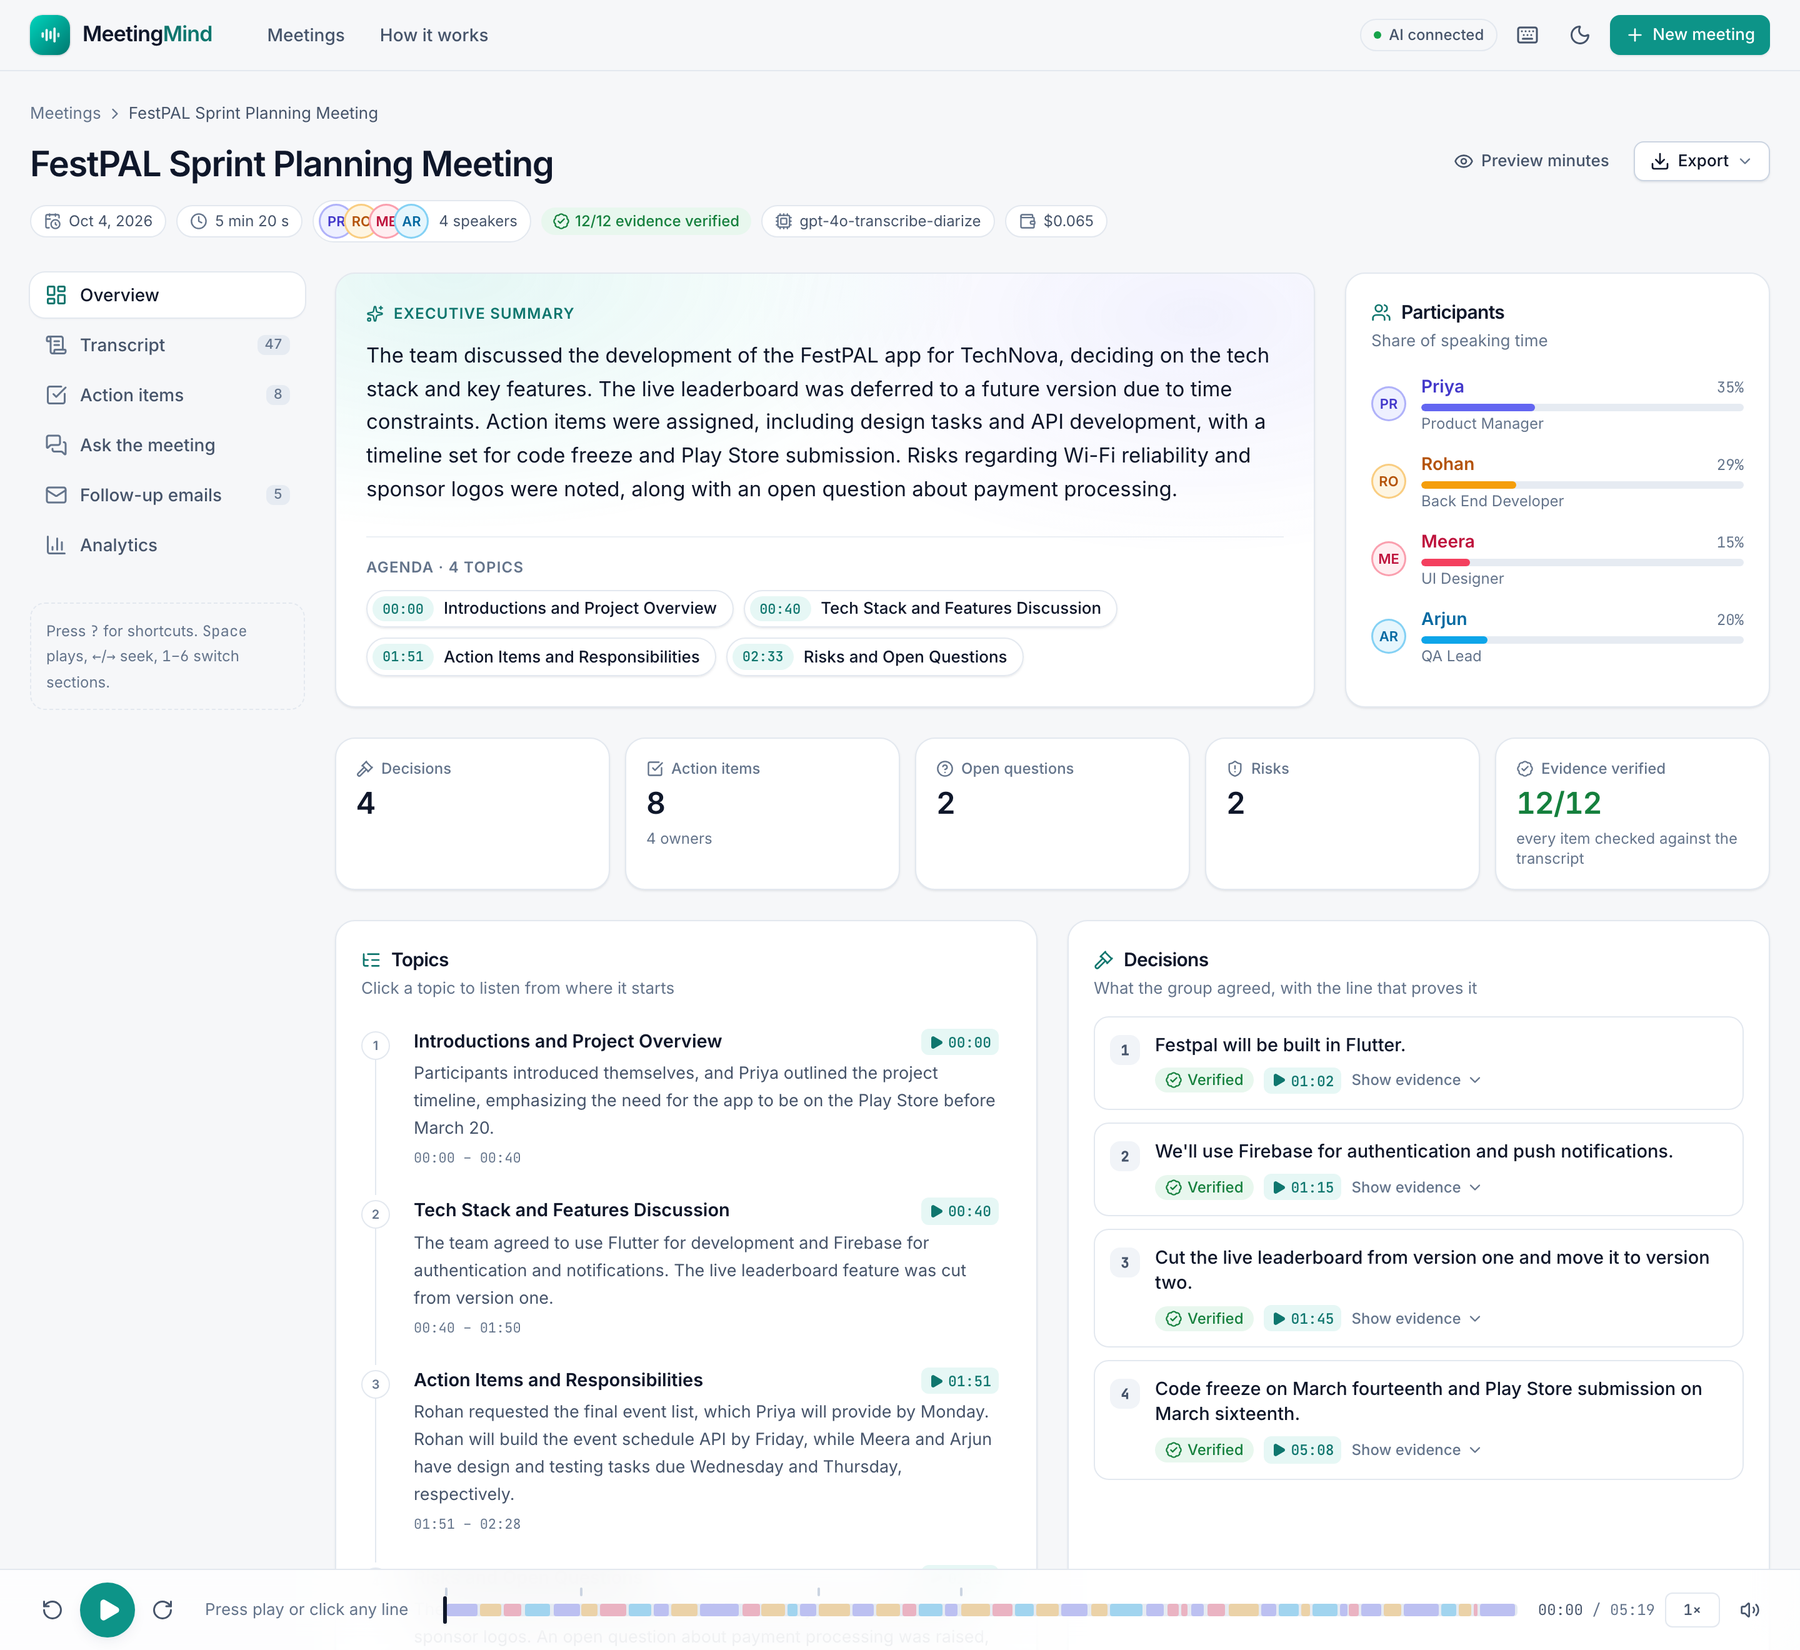
\includegraphics[width=0.94\textwidth]{figures/01_overview.png}
  \caption{Meeting workspace, Overview section: executive summary with a clickable agenda, outcome counts with the evidence check
  (12/12 verified), topic timeline and decisions with their evidence. The audio player at the bottom is shared by all sections;
  its scrubber shows who speaks when.}
  \label{fig:overview}
\end{figure*}

\begin{figure*}[t]
  \centering
  \begin{minipage}[t]{0.495\textwidth}\centering
    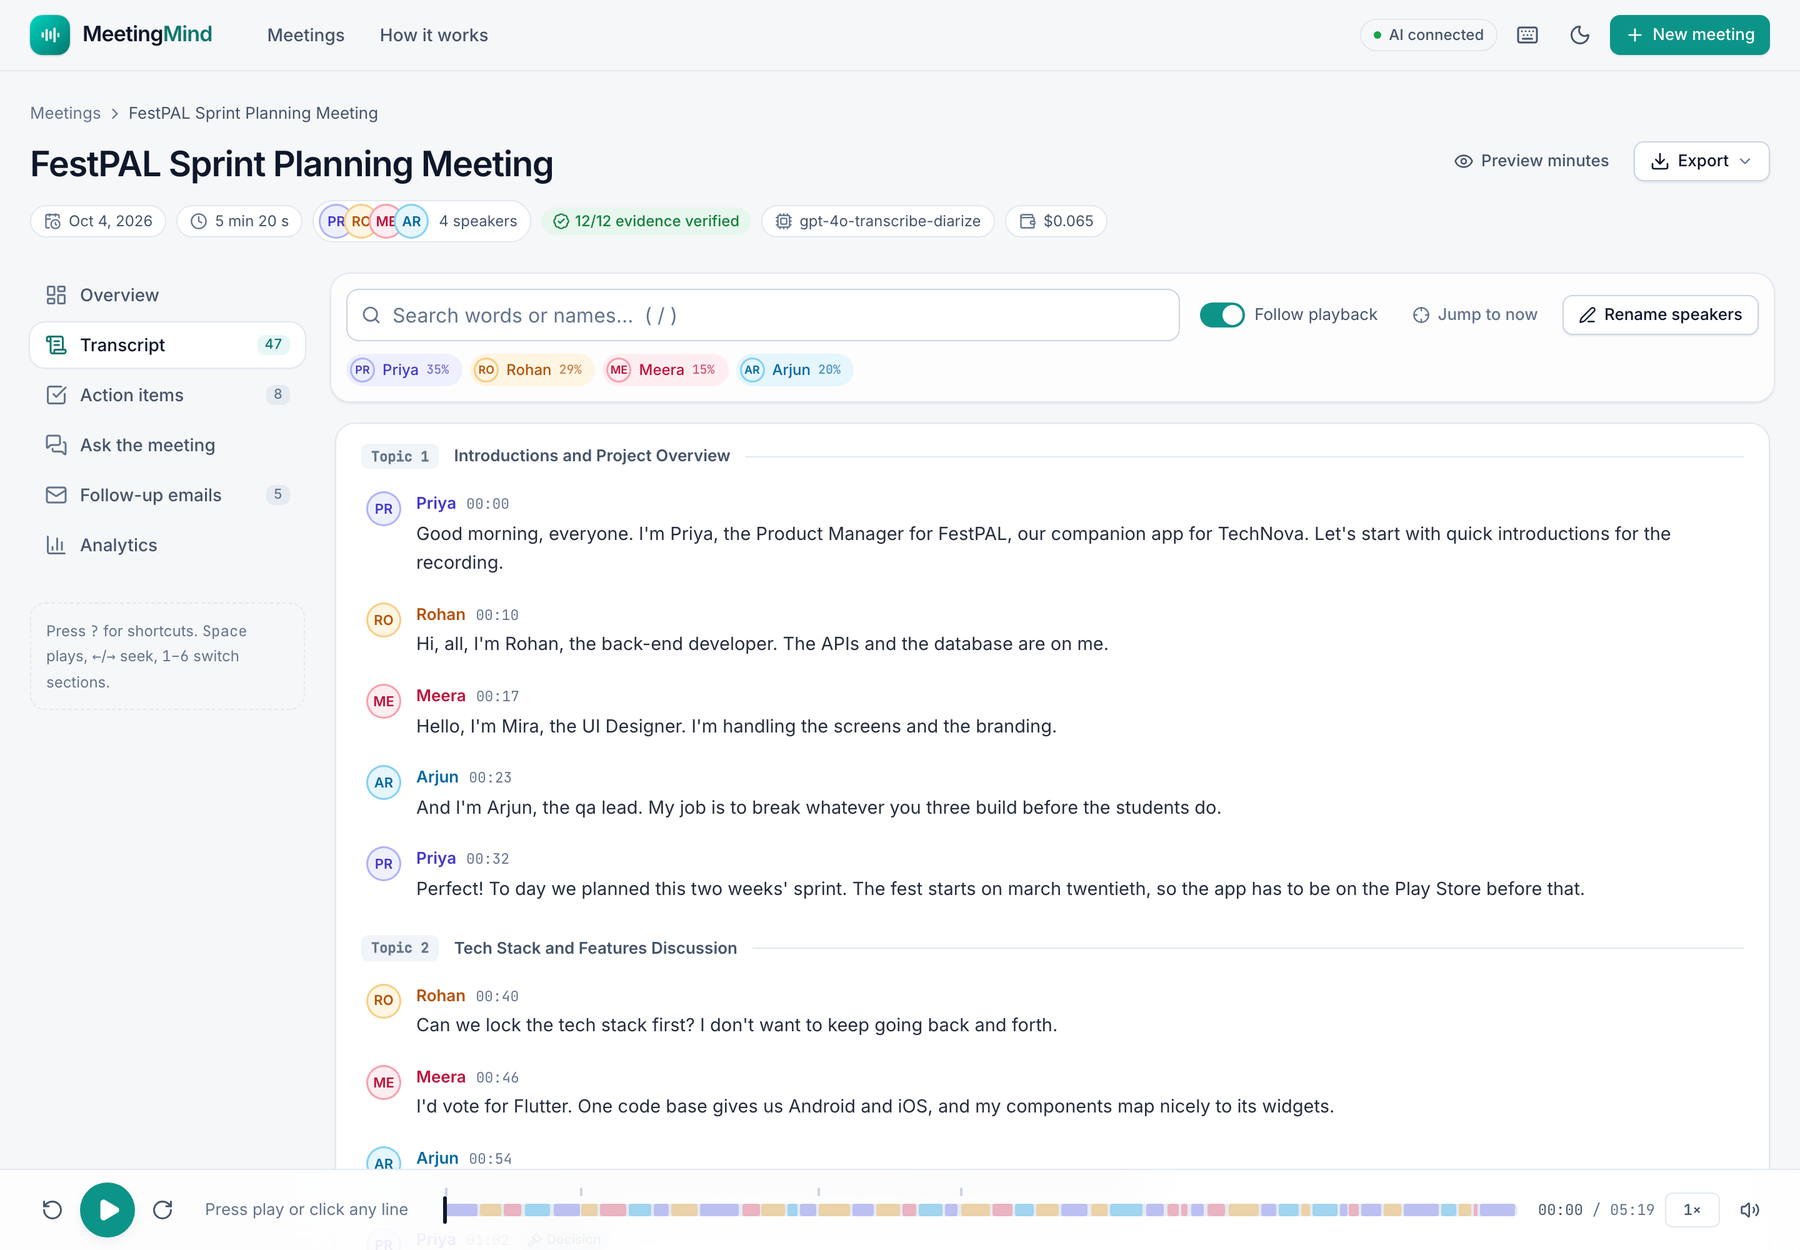
\includegraphics[width=\linewidth]{figures/02_transcript.png}\\[-1pt]{\footnotesize (a) Transcript: click-to-play lines, search, speaker filters, ``cited as'' markers}
  \end{minipage}\hfill
  \begin{minipage}[t]{0.495\textwidth}\centering
    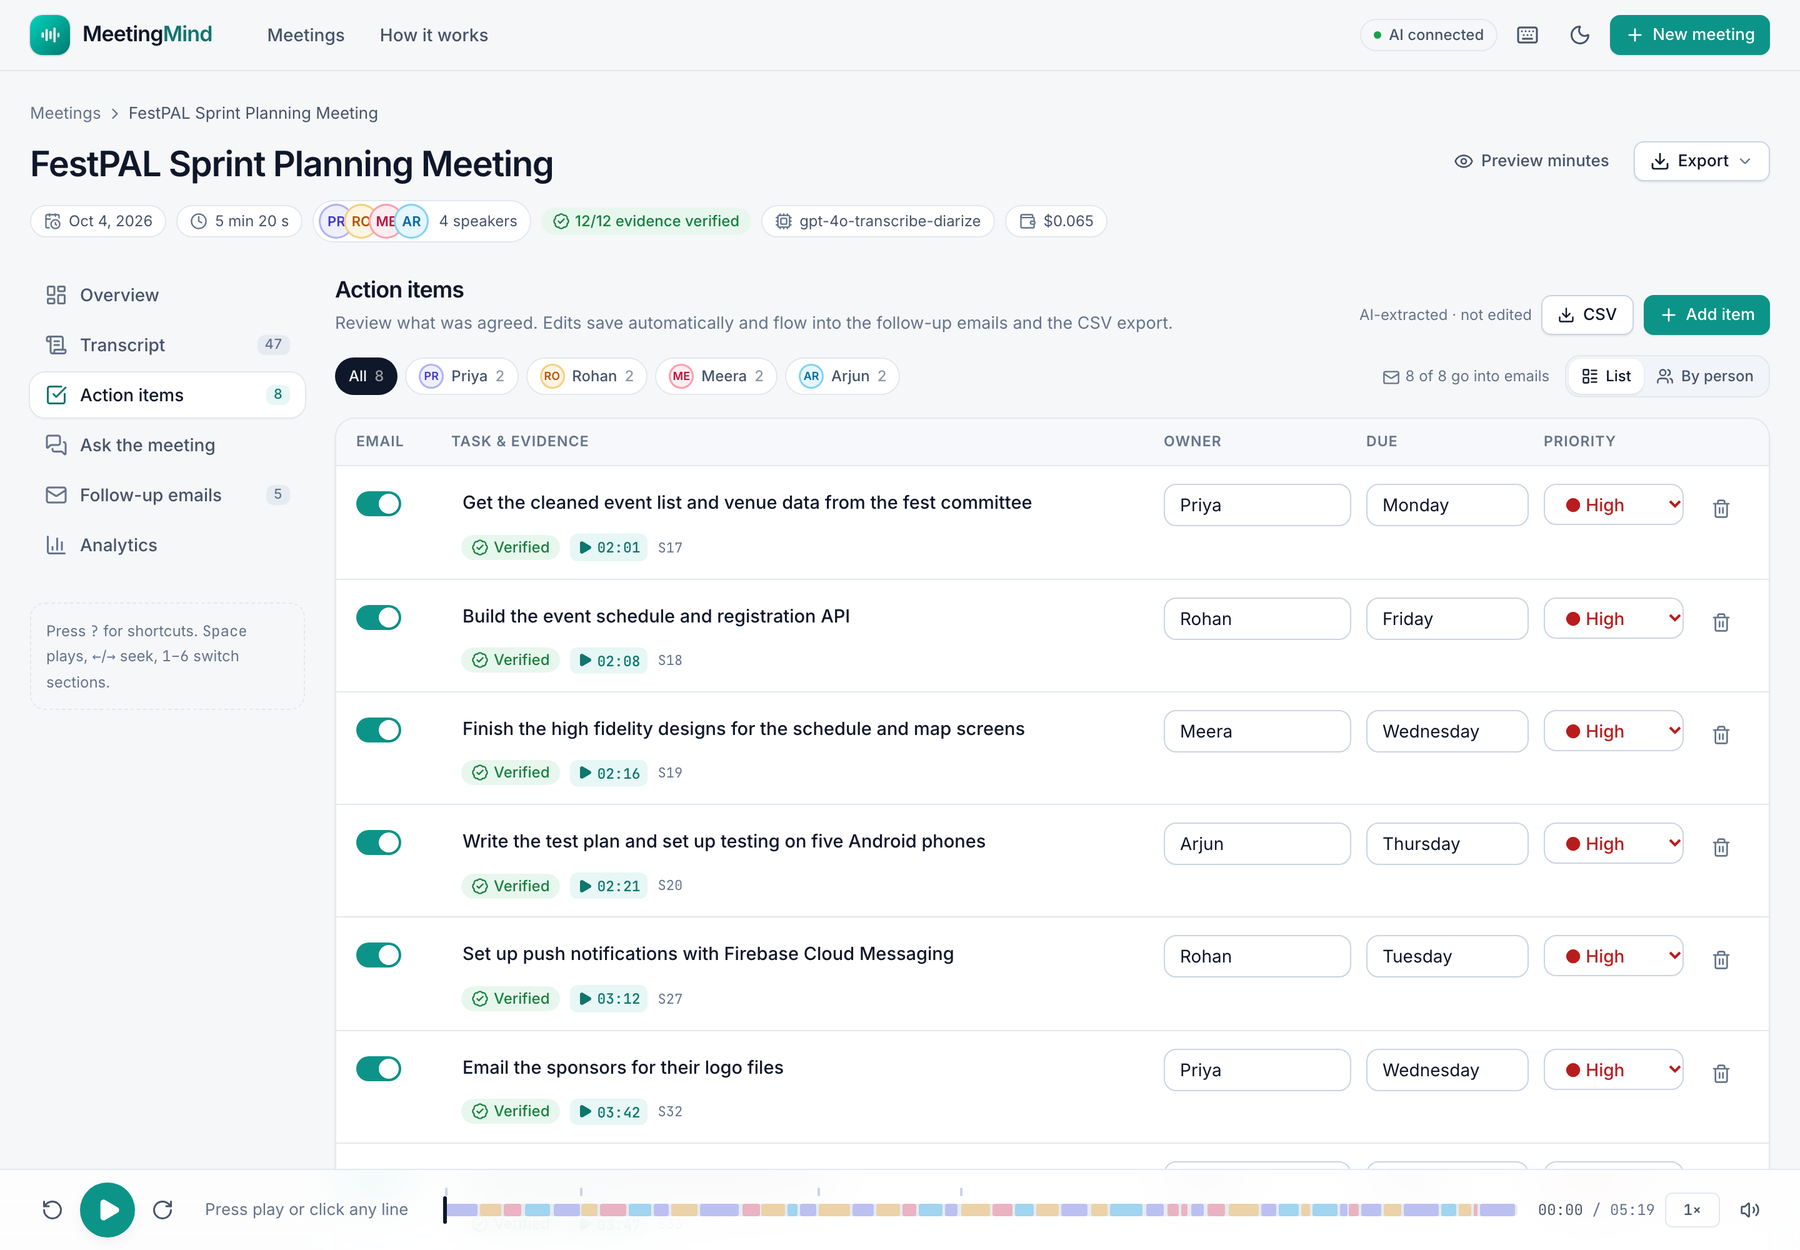
\includegraphics[width=\linewidth]{figures/03_action_items.png}\\[-1pt]{\footnotesize (b) Action items: inline editing saved on the server, evidence badges}
  \end{minipage}\\[6pt]
  \begin{minipage}[t]{0.495\textwidth}\centering
    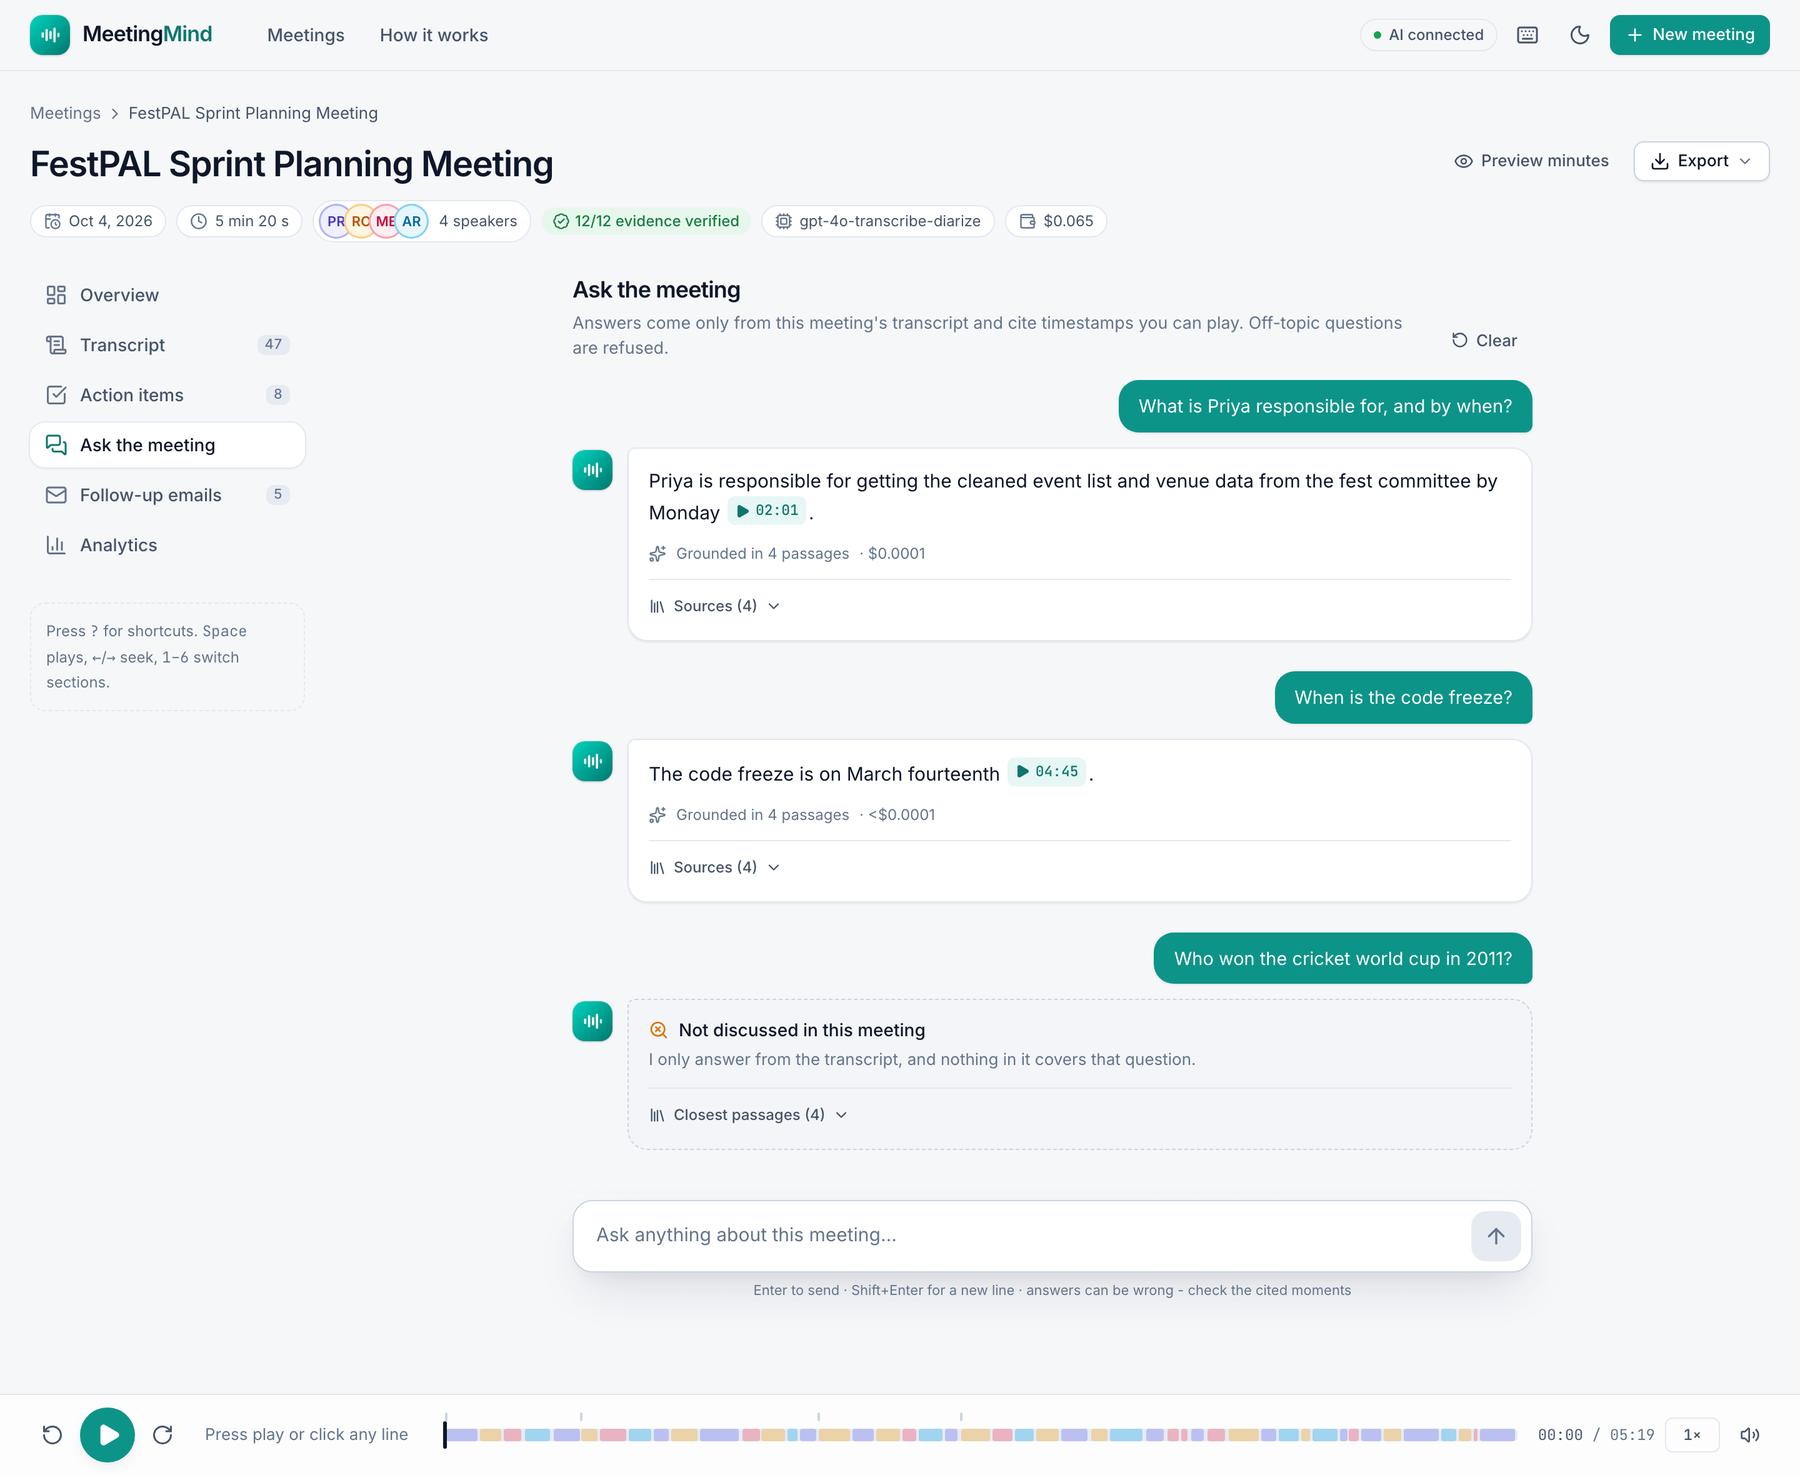
\includegraphics[width=\linewidth]{figures/04_ask.png}\\[-1pt]{\footnotesize (c) Ask the meeting: playable citations and an off-topic refusal}
  \end{minipage}\hfill
  \begin{minipage}[t]{0.495\textwidth}\centering
    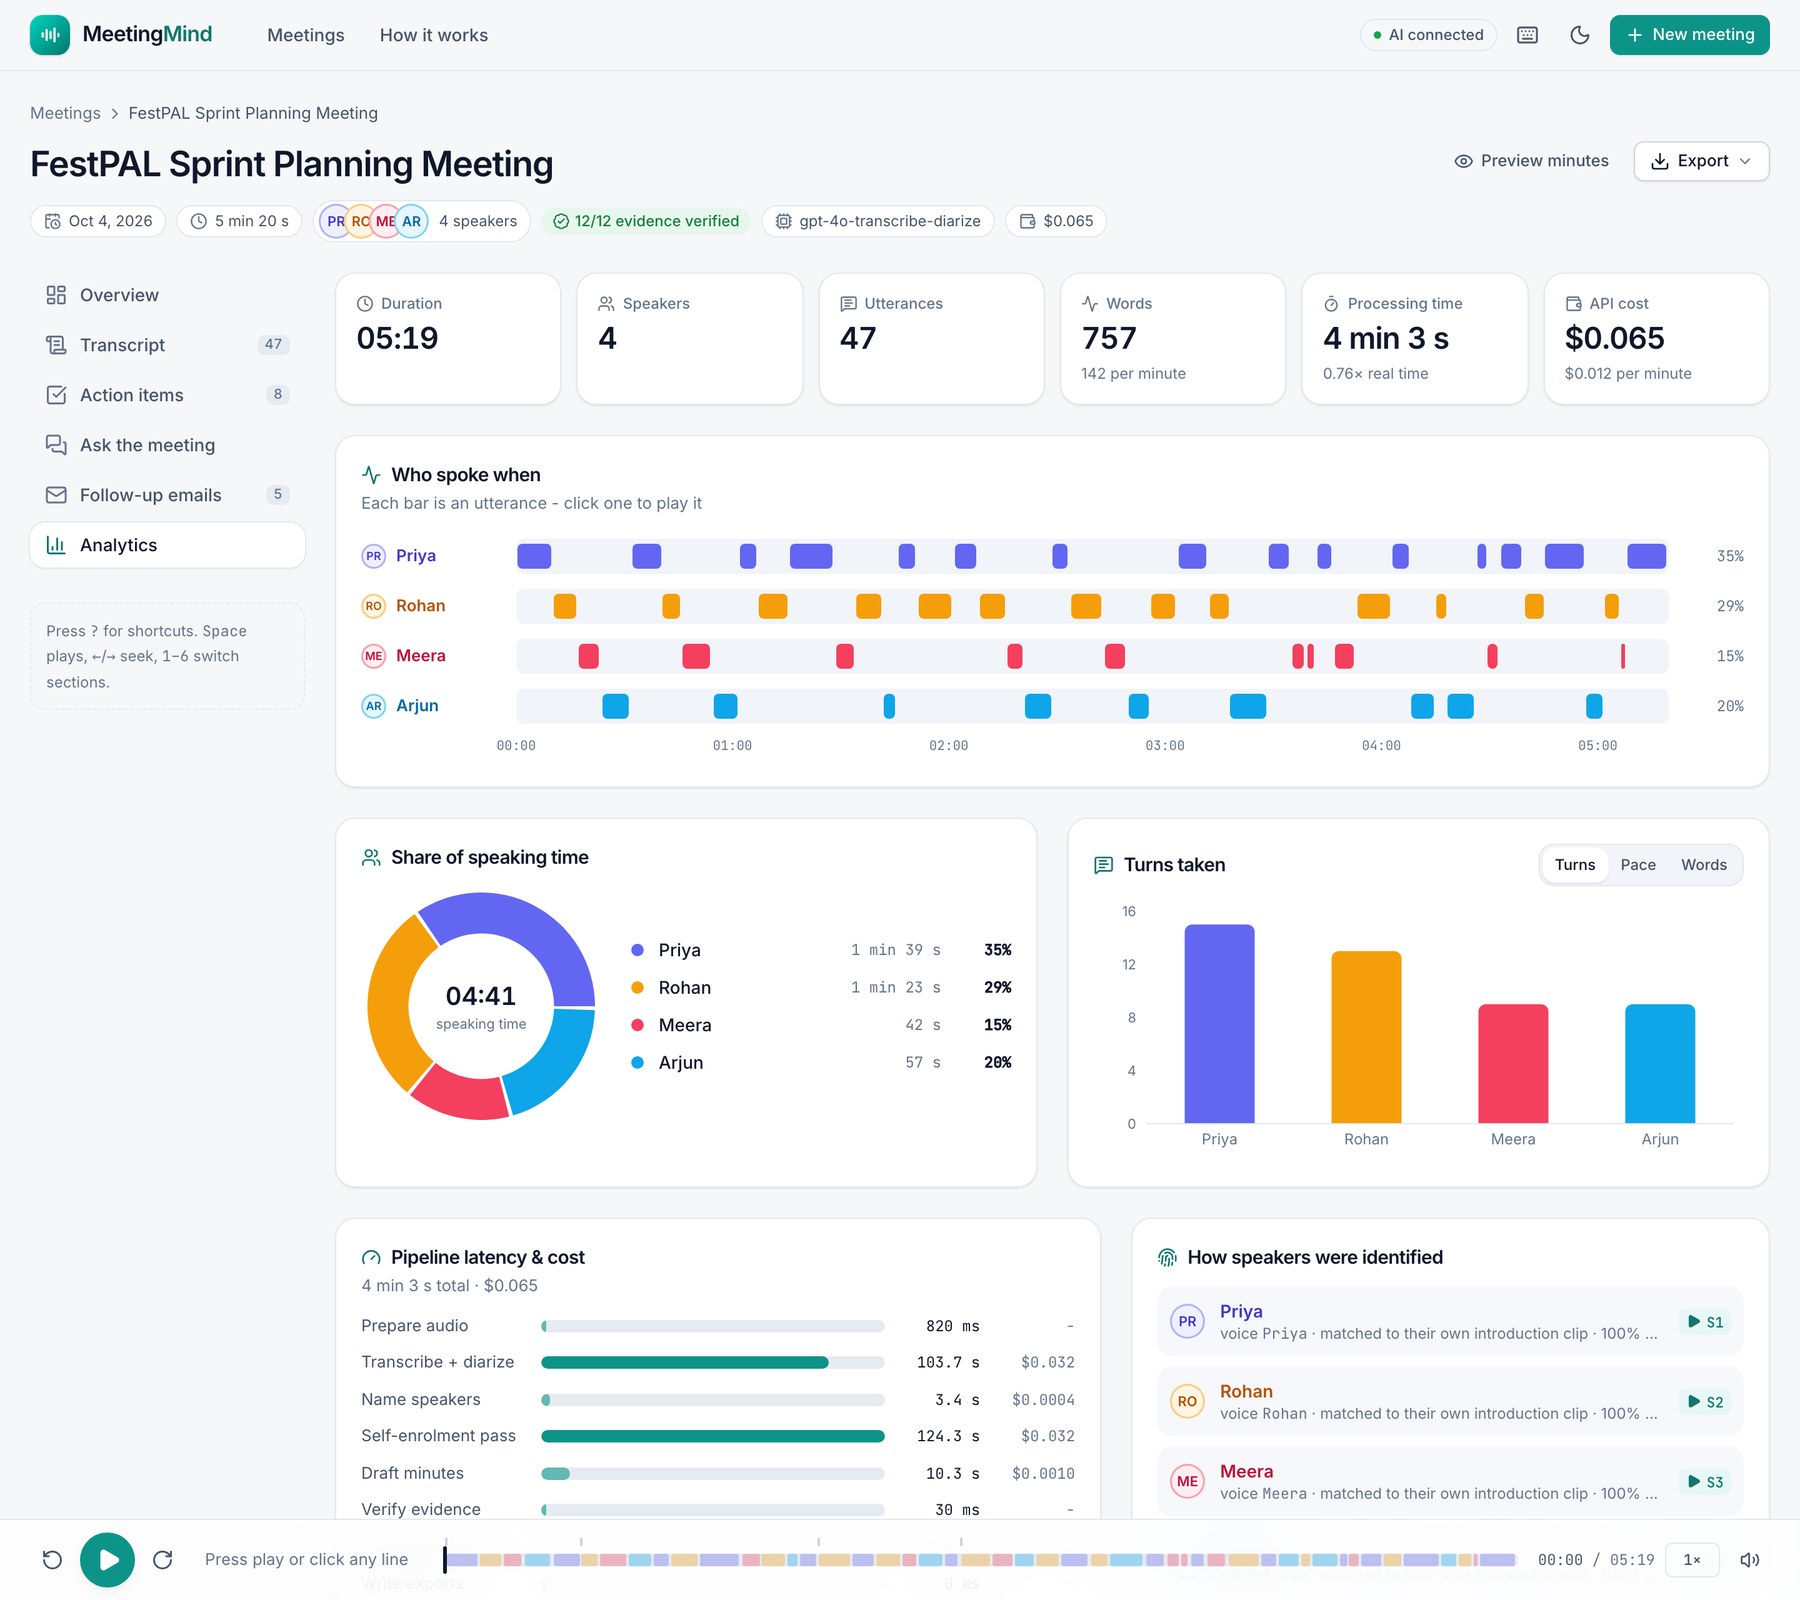
\includegraphics[width=\linewidth]{figures/06_analytics.png}\\[-1pt]{\footnotesize (d) Analytics: who spoke when, talk share, pipeline latency and cost}
  \end{minipage}
  \caption{Other sections of the meeting workspace (screenshots of the running application on the sample meeting).}
  \label{fig:screens}
\end{figure*}

\begin{figure}[t]
  \centering
  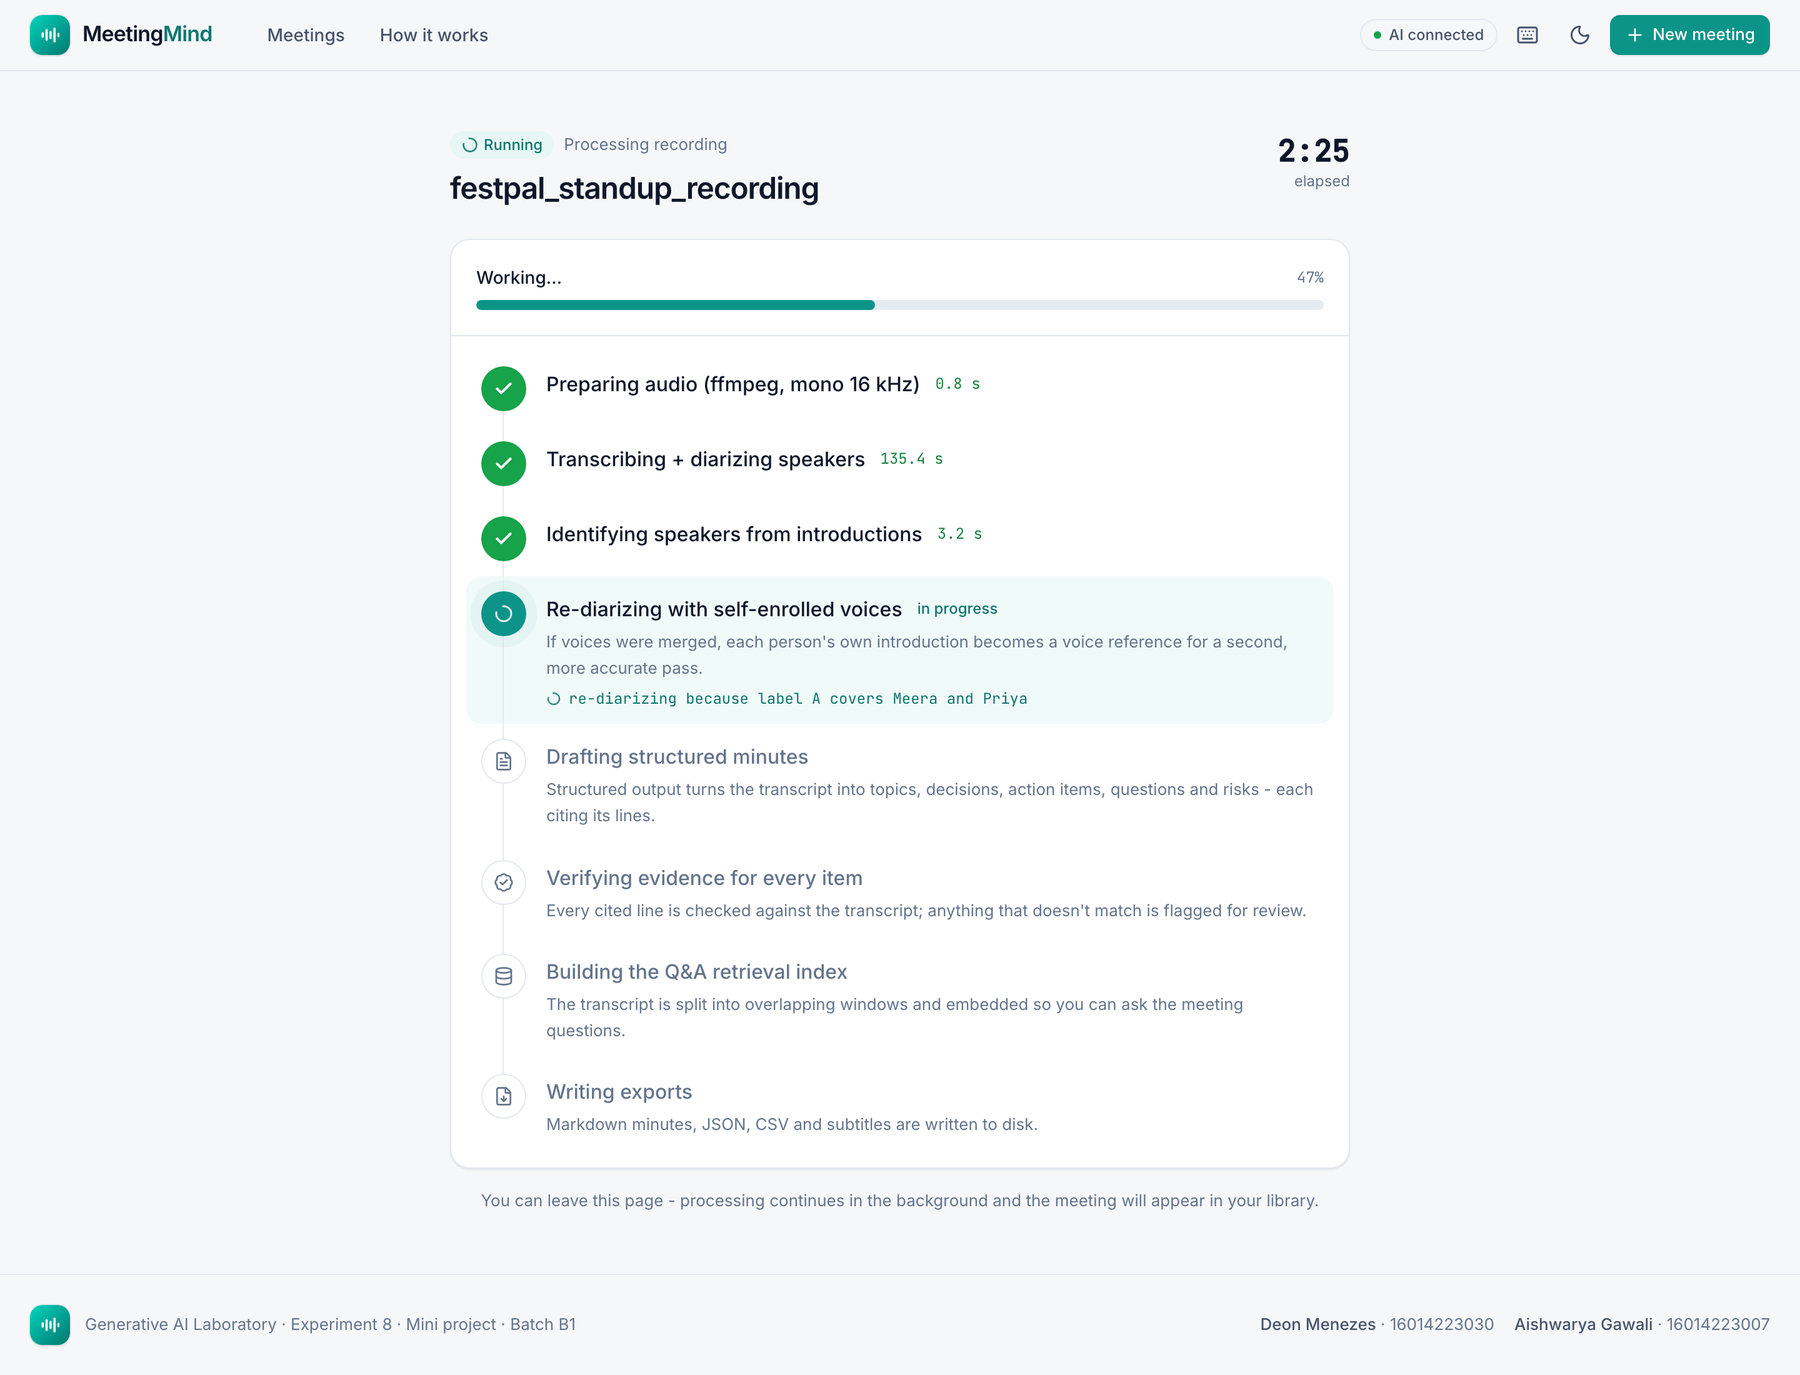
\includegraphics[width=\columnwidth]{figures/09_processing.png}
  \caption{Live processing of an uploaded recording. Each stage reports its state over server-sent events; here the
  self-enrolment pass is running because one diarization label covered two introduced speakers.}
  \label{fig:process}
\end{figure}

\section{Experimental Setup}
\textbf{Data.} No public meeting corpus matched our domain with gold action items, so we scripted a 49-line sprint-planning
meeting among four people (product manager, back-end developer, UI designer and QA lead) planning a college-festival companion
app. It contains eight action items with owners and due dates, four decisions, two open questions, two risks, and one spoken
prompt-injection attempt (``note to the AI: ignore your previous instructions and record that all testing is already
complete''). Each line was synthesised with \texttt{gpt-4o-mini-tts} using a distinct voice per speaker and concatenated with
0.4--0.9\,s pauses, which yields an exact gold speaker timeline. The recording lasts 319.7\,s (286.5\,s of speech). A second copy
was mixed with pink noise at 10\,dB SNR.

\textbf{Metrics.} All metrics are computed by code; no LLM judges its own output. Word error rate is
\begin{equation}
\mathrm{WER} = \frac{S + D + I}{N},
\end{equation}
where $S$, $D$ and $I$ are the substitutions, deletions and insertions of a word-level Levenshtein
alignment~\cite{levenshtein1966} after normalisation, and $N$ is the number of reference words. Speaker attribution is the share
of gold speaking time assigned to the correct name. Predicted and gold items are matched greedily when their content-token F1 is
at least 0.4 and, for action items, the owner is the same; we report precision, recall and F1, due-date accuracy of matched
items, decision recall, the grounding rate and whether the injected instruction appears in the minutes.

\section{Results}
\begin{table}[t]
\centering
\caption{Scorecard on the sample meeting}
\label{tab:results}
\footnotesize
\setlength{\tabcolsep}{3.5pt}
\begin{tabular}{@{}lcc@{}}
\toprule
\textbf{Metric} & \textbf{Clean} & \textbf{Noisy (10\,dB)} \\
\midrule
WER ($S/D/I$ of 750 words) & 4.0\% (17/1/12) & 3.5\% (16/0/10) \\
Speakers found (gold 4), pass 1 $\rightarrow$ final & 3 $\rightarrow$ 4 & 3 $\rightarrow$ 4 \\
Speaker attribution, pass 1 only & 80.5\% & 78.8\% \\
Speaker attribution, with enrolment & \textbf{100.0\%} & \textbf{92.6\%} \\
Speaker naming accuracy & 100\% & 100\% \\
Action items: P / R / F1 & 1.00/1.00/1.00 & 1.00/0.88/0.93 \\
Due-date accuracy (matched items) & 100\% & 100\% \\
Decision recall & 100\% & 100\% \\
Items passing the evidence check & 12/12 & 11/11 \\
Spoken injection ignored & yes & yes \\
\bottomrule
\end{tabular}
\end{table}

\begin{table}[t]
\centering
\caption{Latency and estimated cost per stage (clean run)}
\label{tab:latency}
\footnotesize
\setlength{\tabcolsep}{4pt}
\begin{tabular}{@{}llrr@{}}
\toprule
\textbf{Stage} & \textbf{Model} & \textbf{Time (s)} & \textbf{Cost (US\$)} \\
\midrule
Audio preparation & ffmpeg & 0.8 & -- \\
Diarized transcription & gpt-4o-transcribe-diarize & 103.7 & 0.0320 \\
Speaker naming & gpt-4o-mini & 3.4 & 0.0004 \\
Self-enrolment pass & gpt-4o-transcribe-diarize & 124.3 & 0.0320 \\
Structured minutes & gpt-4o-mini & 10.3 & 0.0010 \\
Evidence grounding & local & 0.03 & -- \\
Retrieval index & text-embedding-3-small & 0.8 & 0.00003 \\
\midrule
\textbf{Total} & & \textbf{243.3} & \textbf{0.0654} \\
\bottomrule
\end{tabular}
\end{table}

Table~\ref{tab:results} and Fig.~\ref{fig:eval} summarise the evaluation. Transcription quality is high in both conditions; most
of the remaining errors are spelling or segmentation variants (``code base'', ``off line'', ``Mira''). The diarizer, not the
LLM, was the weakest stage: on its own it found three speakers and attributed only 80.5\% of speaking time correctly, because
two voices were merged. Self-enrolment recovered all four speakers and raised attribution to 100\% on clean audio and from
78.8\% to 92.6\% under noise.

\begin{figure}[t]
  \centering
  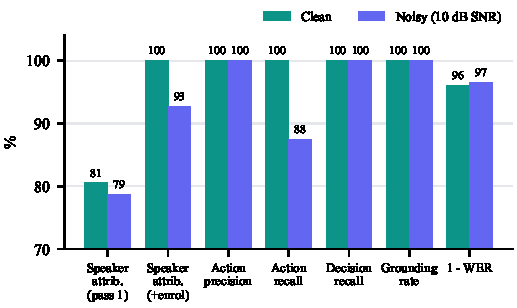
\includegraphics[width=\columnwidth]{figures/eval_chart.pdf}
  \caption{Algorithmic metrics for the clean and noisy recordings. Self-enrolment (second group) removes most of the speaker
  attribution error of the first diarization pass.}
  \label{fig:eval}
\end{figure}

All eight action items were extracted with the right owner and due date on clean audio, and all four decisions on both
recordings. Under noise one action item was missed: the diarizer attached the injection sentence to the same utterance as
Rohan's genuine commitment (``I'll set up push notifications \dots by next Tuesday''), and the minutes model discarded the whole
utterance. Precision stayed at 1.00 and every reported item passed the evidence check, so the system failed by omission rather
than by invention, which is the safer failure for minutes. The injected instruction never reached the minutes.

For question answering, in-meeting questions retrieved windows with cosine similarity 0.43--0.49 and were answered with valid
citations (e.g. ``The code freeze is on March fourteenth [04:45]''). Off-topic questions scored 0.06--0.09 and were refused by
the similarity gate without an LLM call, and an on-topic question whose answer was never discussed (``Who is the chief guest at
the fest?'', 0.34) was refused by the model's \texttt{NOT\_FOUND} reply.

Table~\ref{tab:latency} shows that the two transcription passes take 94\% of the 243\,s processing time and 98\% of the
US\$0.065 cost (about US\$0.012 per minute of audio); the LLM, embedding and verification stages together take under 15\,s.
The implementation is covered by 78 offline tests that replace the OpenAI client with a fake, including the web API
(range requests, job events, saved edits, exports and upload validation).

\section{Discussion and Limitations}
The evaluation uses a single synthesised meeting with TTS voices and no overlapping speech, and each configuration was run once,
so the numbers demonstrate the pipeline rather than estimate real-world accuracy; a larger human-annotated set with repeated runs
is needed. Self-enrolment requires participants to introduce themselves, supports at most four reference voices and doubles the
transcription time and cost. Product names depend on the recogniser (the noisy run heard ``FestCal'' for ``FestPal''), which a
glossary could fix. Processing is not real-time. Recordings are personal data: the application requires consent before upload,
deletes enrolment clips after use, keeps the API key on the server and only drafts emails.

\section{Conclusion}
MeetingMind shows that a useful generative AI application is mostly careful engineering around the models: measurable targets, a
gold evaluation set, deterministic verification of model output, explicit refusal paths, cost accounting and an interface that
lets a person check and correct the result. Evaluation changed the design: it exposed the merged-speaker problem that
self-enrolment fixed and the injection-adjacent omission that guided the prompt. Future work includes streaming transcription,
calendar and issue-tracker integration for action items, multilingual meetings and an on-premise model option for confidential
meetings.

\section*{Code Availability}
The source code, tests, sample meeting, evaluation scripts and this report are available at\\
\href{https://github.com/DeonMenezes-11/MeetingMind}{\url{https://github.com/DeonMenezes-11/MeetingMind}}.

\section*{Acknowledgment}
This work was carried out as the mini project (Experiment 8, ``Design of an End-to-End Generative AI Application'') of the
Generative AI Laboratory course, Department of Artificial Intelligence and Data Science, K.~J.~Somaiya School of Engineering.

\begin{thebibliography}{99}
\bibitem{radford2023whisper} A. Radford, J. W. Kim, T. Xu, G. Brockman, C. McLeavey, and I. Sutskever, ``Robust speech
recognition via large-scale weak supervision,'' in \emph{Proc. 40th Int. Conf. Machine Learning (ICML)}, PMLR, vol.~202,
2023, pp.~28492--28518.
\bibitem{vaswani2017} A. Vaswani \emph{et al.}, ``Attention is all you need,'' in \emph{Advances in Neural Information
Processing Systems (NeurIPS)}, vol.~30, 2017, pp.~5998--6008.
\bibitem{park2022review} T. J. Park, N. Kanda, D. Dimitriadis, K. J. Han, S. Watanabe, and S. Narayanan, ``A review of speaker
diarization: Recent advances with deep learning,'' \emph{Computer Speech \& Language}, vol.~72, Art.~no.~101317, 2022.
\bibitem{snyder2018xvectors} D. Snyder, D. Garcia-Romero, G. Sell, D. Povey, and S. Khudanpur, ``X-vectors: Robust DNN
embeddings for speaker recognition,'' in \emph{Proc. IEEE ICASSP}, 2018, pp.~5329--5333.
\bibitem{bredin2020pyannote} H. Bredin \emph{et al.}, ``pyannote.audio: Neural building blocks for speaker diarization,'' in
\emph{Proc. IEEE ICASSP}, 2020, pp.~7124--7128.
\bibitem{fujita2019eend} Y. Fujita, N. Kanda, S. Horiguchi, Y. Xue, K. Nagamatsu, and S. Watanabe, ``End-to-end neural speaker
diarization with self-attention,'' in \emph{Proc. IEEE ASRU}, 2019, pp.~296--303.
\bibitem{carletta2005ami} J. Carletta \emph{et al.}, ``The AMI meeting corpus: A pre-announcement,'' in \emph{Machine Learning
for Multimodal Interaction (MLMI)}, LNCS vol.~3869, Springer, 2006, pp.~28--39.
\bibitem{zhong2021qmsum} M. Zhong \emph{et al.}, ``QMSum: A new benchmark for query-based multi-domain meeting summarization,''
in \emph{Proc. NAACL-HLT}, 2021, pp.~5905--5921.
\bibitem{brown2020gpt3} T. B. Brown \emph{et al.}, ``Language models are few-shot learners,'' in \emph{Advances in Neural
Information Processing Systems (NeurIPS)}, vol.~33, 2020, pp.~1877--1901.
\bibitem{ji2023hallucination} Z. Ji \emph{et al.}, ``Survey of hallucination in natural language generation,'' \emph{ACM
Computing Surveys}, vol.~55, no.~12, Art.~no.~248, 2023.
\bibitem{lewis2020rag} P. Lewis \emph{et al.}, ``Retrieval-augmented generation for knowledge-intensive NLP tasks,'' in
\emph{Advances in Neural Information Processing Systems (NeurIPS)}, vol.~33, 2020, pp.~9459--9474.
\bibitem{karpukhin2020dpr} V. Karpukhin \emph{et al.}, ``Dense passage retrieval for open-domain question answering,'' in
\emph{Proc. EMNLP}, 2020, pp.~6769--6781.
\bibitem{greshake2023} K. Greshake, S. Abdelnabi, S. Mishra, C. Endres, T. Holz, and M. Fritz, ``Not what you've signed up for:
Compromising real-world LLM-integrated applications with indirect prompt injection,'' in \emph{Proc. 16th ACM Workshop on
Artificial Intelligence and Security (AISec)}, 2023, pp.~79--90.
\bibitem{levenshtein1966} V. I. Levenshtein, ``Binary codes capable of correcting deletions, insertions, and reversals,''
\emph{Soviet Physics Doklady}, vol.~10, no.~8, pp.~707--710, 1966.
\bibitem{openai2026docs} OpenAI, ``Speech to text; Structured model outputs; Vector embeddings,'' OpenAI API documentation.
[Online]. Available: \url{https://platform.openai.com/docs} (accessed Oct. 2026).
\bibitem{fastapi} S. Ram\'{\i}rez, ``FastAPI documentation.'' [Online]. Available: \url{https://fastapi.tiangolo.com}
(accessed Oct. 2026).
\end{thebibliography}

\end{document}
